%-----------------------------------------------------------------------------%
%  DOCUMENT CLASS OPTIONS
%-----------------------------------------------------------------------------%
% The following is a list of the available document class options.
% The first option listed is the default, for more details see
% the "DEFAULT DOCUMENT CLASS OPTIONS" section in utk-class.cls
%   dissertation, thesis
%   12pt, 11pt
%   roman, sans, typewriter
%   onehalfspace, singlespace, doublespace
%   lefttext, justifytext
%   lefttitle, centertitle
%   centerpagenum, rightpagenum
%   noteson, notesoff

%\documentclass[thesis]{utk-class}
\documentclass[dissertation]{utk-class}
%-----------------------------------------------------------------------------%


%-----------------------------------------------------------------------------%
%  PACKAGE CONFIGURATIONS
%-----------------------------------------------------------------------------%
% Fonts - choose at most one
%\usepackage{helvet} % Helvetica (sans)
%\usepackage{avant} % Avant-Garde (sans)
\usepackage{times} % Times (sans/roman)
%\usepackage{lmodern} % Latin Modern (sans/roman)
%\usepackage{tgtermes} % TeX Gyre Termes (roman)
%\usepackage{tgschola} % TeX Gyre Schola (roman)
%\usepackage{palatino} % Palatino (sans/roman)
%\usepackage{courier} % Courier (sans/roman)
%\usepackage{utopia} % Utopia (sans/roman)
%\usepackage{bookman} % Bookman (sans/roman)
%\usepackage{charter} % Charter (roman)

% Bibliography package
%\usepackage{natbib}           % references
\usepackage[numbers]{natbib}  % references with numbering

% Paths where figures are located and allowed file image extensions
\graphicspath{{figures/}{figures/pdf/}{figures/eps/}}
\DeclareGraphicsExtensions{.png,.pdf,.jpg}
%\DeclareGraphicsExtensions{.eps}

% Manually correct bad/special hyphenations
%\hyphenation{op-tical net-works semi-conduc-tor}
%-----------------------------------------------------------------------------%


%-----------------------------------------------------------------------------%
%  GENERAL INFORMATION
%-----------------------------------------------------------------------------%
\title{Analysis on some data using some technique}
\author{Student A. Name} % name as registered in official student records
%\degree{Master of Science}
\degree{Doctor of Philosophy}
\major{Computer Science}
\department{Electrical Engineering and Computer Science}
\university{The University of Tennessee, Knoxville}
\graduationYear{2019}
\graduationMonth{December}
\majorProfessor{Jane P. Doe}
\dean{Dixie L. Thompson}
\committeeMembers{
Member A. Davis,
Member B. Miller,
Member C. Smith
}
%-----------------------------------------------------------------------------%


\begin{document}


%-----------------------------------------------------------------------------%
%  COMMITTEE APPROVAL FORMS
%-----------------------------------------------------------------------------%
%{\singlespacing \makeApprovalPage} % optional, print form
%{\singlespacing \makeApprovalPageE} % optional, electronic form
%-----------------------------------------------------------------------------%


%-----------------------------------------------------------------------------%
%  FRONT-MATTER
%-----------------------------------------------------------------------------%
\clearpage\pagenumbering{roman}
{\onehalfspacing \makeTitlePage}
{\singlespacing \makeCopyrightPage} % optional
\chapter*{Dedication}

\begin{center}
    \vspace*{\fill}
    If the student wishes to dedicate the thesis/dissertation, the dedication
    statement is included on this page. If appropriate, the student may include
    a short quote or other text here. The student may choose to omit the heading
    “Dedication” on this page if the intent of the dedication itself is clear.
    This page is optional.
    \vspace*{\fill}
\end{center} 

 % optional
\chapter*{Acknowledgments} \label{acknowledgments}

The acknowledgments page is used to thank those who have helped in the
process of obtaining the graduate degree. Permission to quote copyrighted
material is listed here, as well as acknowledgment for grants and
special funding. If students must include a disclaimer, stating, for example,
that the views expressed in the thesis or dissertation are not necessarily
the views of the agency or institution that funded or supported the research,
they should do so on this page. This page is optional.
 % optional
\chapter*{Abstract} \label{abstract}

The content of the abstract is determined by the student and committee,
the following information is appropriate: (1) a short statement concerning
the area of investigation, (2) a brief discussion of methods and procedures
used in gathering the data, (3) a condensed summary of the findings, and/or
(4) conclusions reached in the study.

The abstract will be used by the University of Tennessee Libraries in cataloguing
the thesis or dissertation. Therefore, the abstract must NOT exceed 350 words
in length. Furthermore, if the abstract contains any special characters
(those characters not found on typical English-language keyboards) the student
must also write out the term or concept in plain English in square brackets
immediately following the special character. For example: $\pi$ [pi].
If you have questions about what qualifies as a special character, please
check with the thesis/dissertation consultant.

\chapter*{Preface} \label{ch:preface}

A personal statement about the purpose and scope of the thesis/dissertation
could be included in the preface. The tone of the preface, however, must be
academic and appropriate to scholarly work. This page is optional.

 % optional
%-----------------------------------------------------------------------------%


%-----------------------------------------------------------------------------%
%  TABLE OF CONTENTS/TABLE/FIGURES/NOMENCLATURE
%-----------------------------------------------------------------------------%
{\onehalfspacing \tableofcontents}
{\onehalfspacing \listoftables} % if applicable
{\onehalfspacing \listoffigures} % if applicable
{\onehalfspacing \chapter*{List of Abbreviations} \label{abbreviations}

\begin{tabular}{@{}C{1in} L{4.5in}}
AAA & American Anthropology Association \\
APA & American Psychological Association \\
IEEE & Institute of Electrical and Electronics Engineers \\
AI & Artificial intelligence \\
CNN & Convolutional neural networks \\
SaaS & Software as a service \\
R\&D & Research and development \\
UTK & University of Tennessee, Knoxville \\
\end{tabular}
} % if applicable
{\onehalfspacing \chapter*{List of Symbols} \label{symbols}

\begin{tabular}{@{}C{1in} L{4.5in}}
$\phi_p$ & Horizontal stress \\
$\beta$ & Angle between the normal and horizontal planes \\
$\pi$ & Pi \\
$i$ & Imaginary unit \\
$P_2$ & Universal parabolic constant \\
$t_i$ & Time at step $i$ \\
$\Delta\mu$ & Change in energy \\
\end{tabular}
} % if applicable
%-----------------------------------------------------------------------------%


%-----------------------------------------------------------------------------%
%  CHAPTERS
%-----------------------------------------------------------------------------%
\clearpage\pagenumbering{arabic}
\chapter{Introduction} \label{ch:chapter1}

This is a very short guide to an unofficial thesis/dissertation template for the University of Tennessee. It is based on the 2010 thesis specifications but can be easily altered as the guidelines are changed. This template requires a basic knowledge of \LaTeX\ and should cover the basic requirements in terms of required packages and functionality. This is a very short guide to an unofficial thesis/dissertation template for the University of Tennessee. It is based on the 2010 thesis specifications but can be easily altered as the guidelines are changed. This template requires a basic knowledge of \LaTeX\ and should cover the basic requirements in terms of required packages and functionality.

\begin{figure}[b!]
  \centering
  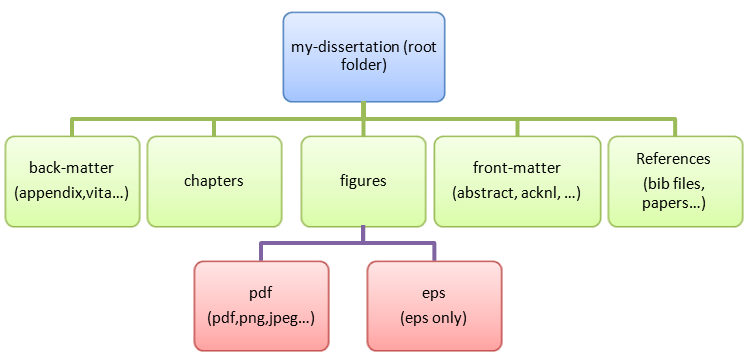
\includegraphics[width=6.5in]{fig01-folder-structure}\\
  \caption{UT thesis template folder structure.}\label{fig:intro-folder-structure}
\end{figure}
The general structure of this template is based on the tree shown in Figure \ref{fig:intro-folder-structure}. The titles of the folders are self descriptive and should guide you to proper file placement. Note that this is only a suggested model that could be modified to fit your own organizational structure.

\begin{verbatim}
%%%%%%%%%%%%%%%%%%%%%%%%%%%%%%%%%%%%%%%%%%%%%%%%%%%%%%%%%%%%%%%%%%%%%%%%%%%
Thesis, color, one side
\documentclass[thesis,monochrome,letterpaper,12pt]{utthesis}
Thesis, monochrome, one side
\documentclass[thesis,monochrome,letterpaper,12pt]{utthesis}
Thesis, color, twoside side (good for binding)
\documentclass[thesis,twoside,letterpaper,12pt]{utthesis}
Thesis, monochrome, twoside side (good for binding)
\documentclass[thesis,monochrome,twoside,letterpaper,12pt]{utthesis}
Dissertation, color, one side
\documentclass[dissertation,letterpaper,12pt]{utthesis}
Dissertation, monochrome, two side
\documentclass[dissertation,twoside,letterpaper,12pt]{utthesis} . . .
%%%%%%%%%%%%%%%%%%%%%%%%%%%%%%%%%%%%%%%%%%%%%%%%%%%%%%%%%%%%%%%%%%%%%%%%%%%
\end{verbatim}

\section{Theorem environments}
This template contains predefined theorem, lemma, and corollary environments. For example
\begin{theorem}[First theorem]\label{thm:theorem-a}
    This is an example theorem.
\end{theorem}
\begin{proof}[Proof for theorem] \ref{thm:theorem-a}
    This is the proof for this theorem.
\end{proof}
\begin{lemma}[First lemma]
    This is the first lemma.
\end{lemma}
\begin{corollary}
    This is the first corollary.
\end{corollary}

\subsection{Single figures}
For more information, check: \href{http://en.wikibooks.org/wiki/LaTeX/Floats,_Figures_and_Captions}{http://en.wikibooks.org/wiki/LaTeX/Floats,\_Figures\_and\_Captions}

\subsubsection{Testing}
In this part we tested some stuff.

\subsection{Multipart figures}
For multipart figures, you need to use the package "subfig". here's an example
\begin{figure}[h!]
        \centering
        \subfloat[Circle]{\label{fig:figure-a}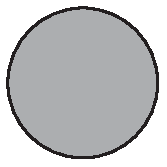
\includegraphics[width=1.1in]{fig02a-circle}}
        \subfloat[Rectangle]{\label{fig:figure-b}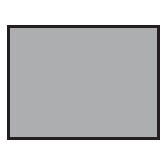
\includegraphics[width=1.1in]{fig02b-rectangle}}
        \subfloat[Cube]{\label{fig:figure-c}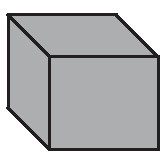
\includegraphics[width=1.1in]{fig02c-cube}}
        \caption{Geometric shapes.}
        \label{fig:multipart-figure}
\end{figure}
To add some space between the figures above, one can use the usual spacing commands such as ``qquad''
\begin{figure}[h!]
        \centering
        \subfloat[Circle]{\label{fig:figure-a}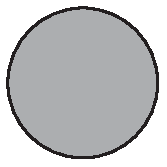
\includegraphics[width=1.1in]{fig02a-circle}} \qquad
        \subfloat[Rectangle]{\label{fig:figure-b}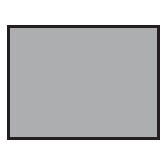
\includegraphics[width=1.1in]{fig02b-rectangle}}\qquad
        \subfloat[Cube]{\label{fig:figure-c}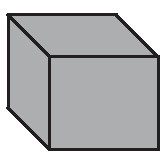
\includegraphics[width=1.1in]{fig02c-cube}}\qquad
        \caption{Geometric shapes.}
        \label{fig:multipart-figure}
\end{figure} 

\chapter{Experiments} \label{chapter2}

This is a citation~\cite{utk:idr2016optimization}.
This is a very short guide to an unofficial thesis/dissertation template
for the University of Tennessee.
It is based on the 2017 thesis specifications but can be easily altered
as the guidelines are changed.
This template requires a basic knowledge of \LaTeX\ and should cover
the basic requirements in terms of required packages and functionality.


\chapter{Results} \label{ch:chapter3}

This is a very short guide to an unofficial thesis/dissertation template for the University of Tennessee. It is based on the 2010 thesis specifications but can be easily altered as the guidelines are changed. This template requires a basic knowledge of \LaTeX\ and should cover the basic requirements in terms of required packages and functionality.


\chapter{Conclusions} \label{ch:conclusions}

This is a very short guide to an unofficial thesis/dissertation template for the University of Tennessee. It is based on the 2010 thesis specifications but can be easily altered as the guidelines are changed. This template requires a basic knowledge of \LaTeX\ and should cover the basic requirements in terms of required packages and functionality.


%-----------------------------------------------------------------------------%


%-----------------------------------------------------------------------------%
%  BIBLIOGRAPHY
%-----------------------------------------------------------------------------%
\makeBibliography{List of References}
%\bibliographystyle{apalike} % APA
\bibliographystyle{ieeetr} % IEEE Transactions
{\onehalfspacing \bibliography{utk-refs}}
%-----------------------------------------------------------------------------%


%-----------------------------------------------------------------------------%
%  BACK-MATTER
%-----------------------------------------------------------------------------%
\initializeAppendix[1]{Appendices} % if applicable
\chapter{Safety} \label{appendixA}

Here is a math equation: $y = mx + b$\\
The above equation represents a line.

\section{An appendix section} \label{appAsect}

This is a section in Appendix A.

\subsection{An appendix subsection} \label{appAsubsect}

This is a subsection in Appendix A.

\subsubsection{An appendix subsubsection} \label{appAsubsubsect}

This is a subsubsection in Appendix A.

\subsubsection{Another appendix subsubsection} \label{appAsubsubsect2}

This is another subsubsection in Appendix A.
 % if applicable
\chapter{SIMD} \label{appendixB}

This is another appendix for testing format.

\section{Another section} \label{appBsect}

This is a section in Appendix B.
 % if applicable
\finalizeAppendix % restores pre-appendix environment, used with \initializeAppendix

\chapter*{Vita} \label{ch:vita}

The vita should be written in narrative form, not resume or curriculum vitae form.
It should contain appropriate academic and professional information about the
author/student. Because copies of the manuscript will be available to the public,
personal information, such as the student's address or phone number, should not
be included.


%-----------------------------------------------------------------------------%


\end{document}

